\documentclass[12pt, a4paper]{article}
\usepackage{amsmath, amsfonts}
\usepackage[utf8]{inputenc}
\usepackage[russian]{babel}
\usepackage{graphicx}
\usepackage{wrapfig}
\usepackage{float}
\usepackage{geometry}
\usepackage[indentfirst,compact,topmarks,calcwidth,pagestyles]{titlesec}
\usepackage{verbatim}
\usepackage{titletoc}
\usepackage{cmap}
\usepackage{hyperref}
%\geometry{verbose, a4paper, top=2cm, bottom=2cm, left=3cm, right=1cm}
% Параметры страницы
\textheight=24cm
\textwidth=16cm
\oddsidemargin=5mm
\evensidemargin=-5mm
\marginparwidth=36pt
\topmargin=-1cm
\footnotesep=3ex
%\flushbottom
\raggedbottom
\tolerance 3000
% подавить эффект ``висячих стpок''
\clubpenalty=10000
\widowpenalty=10000
\usepackage[T2A]{fontenc}


\begin{document}

\begin{titlepage}
\begin{center}
    Московский государственный университет имени М. В. Ломоносова

    \bigskip
    
\includegraphics[width=50mm]{msu.eps}

    \bigskip
    Факультет Вычислительной Математики и Кибернетики\\
    Кафедра Общей Математики\\[10mm]

    \textsf{\large\bfseries
        КУРСОВАЯ РАБОТА СТУДЕНТА 427 ГРУППЫ\\[10mm]
        Решение задачи диффузии-конвекции в жидкости с пульсирующим источником
    }\\[10mm]

    \begin{flushright}
        \parbox{0.5\textwidth}{
            Выполнил:\\
            студент 4 курса 427 группы\\
            \emph{Е. Ю. Пышнограев}\\[5mm]
            Научный руководитель:\\
            д.ф-м.н., профессор\\
            \emph{М. М. Хапаев}
        }
    \end{flushright}

    \vspace{\fill}
    Москва, 2013
\end{center}
\end{titlepage}

\newpage
\begin{abstract}
  В данной работе рассматривается процесс конвективной диффузии вещества в неоднородной среде, состоящей из двух слоев с различными
  физическими и геометрическими параметрами. Показано, как может быть применен метод конечных интегральных преобразований к решению этой задачи.
  Получен окончательный ответ и выделены основные этапы его вычисления. Приведены возникающие при решении трудности и показаны
  на конкретном примере. Приведенная схема может быть применена к нахождению решений более сложных процессов в различных телах больших размерностей.
\end{abstract}

\newpage
\renewcommand{\contentsname}{Содержание}
\tableofcontents

\newpage
\section{Введение}
При работе с многими процессами диффузионного типа возникает необходимость решения уравнений
в частных производных с кусочно-постоянными коэффициентами.
На практике часто используется метод разностных схем, который находит численное решение уравнения при
заданных начальных и граничных условиях.

Но помимо получения численного решения часто необходимо понимать как ведет себя искомая функция, а численные методы не позволяют получить ее в общем виде.
В связи с этим предлагается использовать метод конечных интегральных преобразований.
Указанный метод позволяет получить аналитическое решение задачи путем построения полной ортогональной
системы собственных функций.

В данной работе рассматриваются особенности нахождения такой системы, ее применение для решения исходной задачи
и возникающие при этом трудности.

\section{Постановка задачи}
\begin{wrapfigure}{r}{0.4\textwidth}
  \centering
  \label{fig1}
  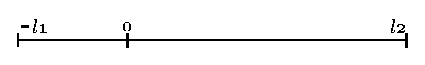
\includegraphics[width=0.38\textwidth]{fig1.eps}
  \\
  \caption{Рассматриваемый отрезок}
\end{wrapfigure}
В данной работе решается задача диффузии-конвекции для одномерной конечной двухслойной области, которая схематически показана на Рис.~1. Для удобства граница раздела слоев помещена в начало координат.

Математическая постановка задачи состоит в следующем: требуется решить уравнение в частных производных
\begin{equation}
 u_t = wu_x + a^2 u_{xx} 
 \label{eq:12}
\end{equation}
с однородным начальным условием
\begin{equation}
 u(x,0) = 0 
\end{equation}
а также внешними и общими граничными условиями 
\begin{equation}
  \left\{
  \begin{aligned}
    & u(-l_1,t) = 1 - \cos \omega t, \\
    & u_x(l_2,t) = 0, \\
    & u(-0, t) = u(+0, t), \\
    & a_1^2 u_{x}(-0, t) = a_2^2 u_{x}(+0, t), \\
  \end{aligned}
  \right.
\end{equation}
где $a(x)$, $w(x)$ --- кусочно-постоянные коэффициенты диффузии и скорости осаждения соответственно:
\begin{equation}
  a=a(x)=\left\{ 
    \begin{aligned}
      & a_1\ \text{при}\ x \in [-l_1;0), \\
      & a_2\ \text{при}\ x \in [0;l_2], \\
    \end{aligned}
\right.
\end{equation}
\begin{equation}
  w=w(x)=\left\{ 
    \begin{aligned}
      & w_1\ \text{при}\ x \in [-l_1;0), \\
      & w_2\ \text{при}\ x \in [0;l_2]. \\
    \end{aligned}
\right.
\end{equation}
\section{Основная часть}
\subsection{Переход к однородным граничным условиям}
Для перехода к однородным граничным условиям производим замену
\begin{equation}
  u(x,t) = U(x,t) + (1 - \cos \omega t).
\end{equation}
В результате приходим к новому уравнению, начальному и граничным условиям
\begin{equation}
  U_t(x,t) = w U_x(x,t) + a^2 U_{xx}(x,t) - \omega\sin\omega t,
  \label{eq:14}
\end{equation}
\begin{equation}
  U(x,0) = 0,
\end{equation}
\begin{equation}
  \left\{
  \begin{aligned}
    & U(-l_1,t) = 0, \\
    & U_x(l_2,t) = 0, \\
    & U(-0, t) = U(+0, t), \\
    & a_1^2 U_{x}(-0, t) = a_2^2 U_{x}(+0, t). \\
  \end{aligned}
  \right.
  \label{eq:15}
\end{equation}
\subsection{Разделение переменных}
Пусть $ U(x,t)=\theta(t)\varphi(x) $, тогда
\begin{equation}
  \frac{\theta'}{\theta}=\frac{a^2\varphi''+w\varphi'}{\varphi}=s.
  \label{eq:1}
\end{equation}
Константа $ s $ не может быть положительной, в противном случае $\lim\limits_{t \rightarrow \infty}\theta(t) \ne 0$, что противоречит физическому смыслу задачи. Ввиду этого, можно принять
\begin{equation}
  s=-\lambda^2.
  \label{eq:2}
\end{equation}
\subsection{Задача Штурма--Лиувилля}
\subsubsection{Исключение конвективного слагаемого}
Из (\ref{eq:1}) и (\ref{eq:2}) следует задача Штурма--Лиувилля для $\varphi(x)$:
\begin{equation}
  a^2 \varphi''(x) + w \varphi'(x) + \lambda^2\varphi(x)=0 \\
\end{equation}
с внешними граничными условиями и условиями сопряжения:
\begin{equation}
  \left\{
  \begin{aligned}
    & \varphi_1(-l_1) = 0, \\
    & \varphi_2'(l_2) = 0, \\
и   & \varphi_1(0) = \varphi_2(0), \\
    & a_1^2 \varphi_1'(0) = a_2^2 \varphi_2'(0). \\
  \end{aligned}
  \right.
  \label{eq:16}
\end{equation}
Здесь
\begin{equation}
  \varphi(x)=\left\{ 
    \begin{aligned}
      & \varphi_1(x)\ \text{при}\ x \in [-l_1;0), \\
      & \varphi_2(x)\ \text{при}\ x \in [0;l_2]. \\
    \end{aligned}
\right.
\end{equation}

Для того чтобы исключить из уравнения слагаемое $w\varphi'(x)$, производим замену 
\begin{equation}
  \varphi(x) = \psi(x) e^{- \mu x},\ \text{где}\ \mu=\mu(x) = \left\{
    \begin{aligned}
      & \mu_1 = \frac{w_1}{2a_1^2}\ \text{при}\ x \in [-l_1;0), \\
      & \mu_2 = \frac{w_2}{2a_2^2}\ \text{при}\ x \in [0;l_2]. \\
    \end{aligned}
    \right.
\end{equation}
В итоге получаем новое уравнение
\begin{equation}
  a^2\psi''(x) + (\lambda^2 - \mu^2a^2) \psi(x) = 0
  \label{eq:3}
\end{equation}
и новые граничные условия
\begin{equation}
  \left\{
  \begin{aligned}
    & \psi_1(-l_1) = 0, \\
    & \psi_2'(l_2) - \mu\psi_2(l_2) = 0, \\
    & \psi_1(0) = \psi_2(0), \\
    & a_1^2(\psi_1'(0) - \mu\psi_1(0)) =  a_2^2(\psi_2'(0) - \mu\psi_2(0)). \\
  \end{aligned}
  \right.
  \label{}
\end{equation}

Пусть для определенности $\mu_1 \le \mu_2$. Тогда для нахождения собственных чисел $\lambda$ необходимо рассмотреть три отрезка. Собственным числам из разных отрезков будет соответствовать разный вид собственных функций
\begin{enumerate}
  \item $ 0 \le \lambda \le \mu_1a_1, $
  \item $ \mu_1a_1 < \lambda \le \mu_2a_2, $
  \item $ \mu_2a_2 < \lambda < \infty. $
\end{enumerate}
\subsubsection{Нахождение собственных чисел и собственных функций}
1.\ $ 0 \le \lambda \le \mu_1a_1$. Собственные функции $\psi$ будут иметь вид:
\begin{equation}
  \begin{aligned}
    \psi_1(x) = A_1 \ch \gamma_1x + B_1 \sh \gamma_1x, \\
    \psi_2(x) = A_2 \ch \gamma_2x + B_2 \sh \gamma_2x.
  \end{aligned}
  \label{eq:5}
\end{equation}
Где 
\begin{equation}
  \begin{aligned}
    \gamma_1 = \gamma_1(\lambda) = \sqrt{- \frac{\lambda^2}{a_1^2} + \mu_1}, \\
    \gamma_2 = \gamma_2(\lambda) = \sqrt{- \frac{\lambda^2}{a_2^2} + \mu_2}.
  \end{aligned}
\end{equation}
Константы $A_1$, $A_2$, $B_1$, $B_2$ определяем из граничных условий. Используя граничные условия, получим:
\begin{equation}
  \left\{  
  \begin{aligned}
    & A_1 \ch \gamma_1l_1 - B_1 \sh \gamma_1l_1 = 0, \\
    & A_2 (\gamma_2\sh \gamma_2l_2 - \mu_2\ch \gamma_2l_2) + B_2 (\gamma_2\ch \gamma_2l_2 - \mu_2\sh \gamma_2l_2) = 0, \\
    & A_1 = A_2, \\
    & A_1 (-\mu_1a_1^2) + B_1 (\gamma_1a_1^2) = A_2 (-\mu_2a_2^2) + B_2 (\gamma_2a_2^2).
  \end{aligned}
  \right.
  \label{eq:4}
\end{equation}
Чтобы найти ненулевые коэффициенты $A_i$, $B_i$, необходимо, чтобы определитель системы уравнений (\ref{eq:4}) относительно $A_i$, $B_i$ был равен нулю. В результате получим уравнение для $\lambda$:
\begin{equation}
  \det \left(  
  \begin{smallmatrix}
    \ch(\gamma_1(\lambda) l_1) & 0 & -\sh(\gamma_1(\lambda) l_1) & 0 \\
    0 & \gamma_2(\lambda) \sh(\gamma_2(\lambda) l_2)-\ch(\gamma_2(\lambda) l_2) \mu_2 & 0 & \gamma_2(\lambda) \ch(\gamma_2(\lambda) l_2)-\sh(\gamma_2(\lambda) l_2) \mu_2 \\
    1 & -1 & 0 & 0 \\
    -a_1^2 \mu_1 & a_2^2 \mu_2 & a_1^2 \gamma_1(\lambda) & -a_2^2 \gamma_2(\lambda) \\
  \end{smallmatrix}
  \right) = 0,
\end{equation}
или в развернутом виде
\begin{equation}
  \begin{aligned}
  & -\sh(\gamma_1(\lambda) l_1) ((a_2^2 \mu_2-a_1^2 \mu_1) (\gamma_2(\lambda) \ch(\gamma_2(\lambda) l_2)-\sh(\gamma_2(\lambda) l_2) \mu_2)+a_2^2 \gamma_2(\lambda)- \\
  & -(\gamma_2(\lambda) \sh(\gamma_2(\lambda) l_2)-\ch(\gamma_2(\lambda) l_2) \mu_2))-a_1^2 \gamma_1(\lambda) \ch(\gamma_1(\lambda) l_1) \times \\
  & \times (\gamma_2(\lambda) \ch(\gamma_2(\lambda) l_2)-\sh(\gamma_2(\lambda) l_2) \mu_2) = 0.
  \end{aligned}
  \label{eq:19}
\end{equation}
После определения собственных чисел, из системы (\ref{eq:4}) находим коэффициенты $A_i$, $B_i$
\begin{equation}
  \begin{aligned}
    & A_1 = A_2 = \sh \gamma_1l_1, \\
    & B_1 = \ch \gamma_1l_1, \\
    & B_2 = \frac{\sh (\gamma_1l_1) (-\mu_1 a_1^2 + \mu_2 a_2^2) + \ch (\gamma_1l_1) \gamma_1 a_1^2}{\gamma_2a_2^2}.
  \end{aligned}
\end{equation}
Таким образом, найден набор собственных функций (\ref{eq:5}), соответствующий отрезку $ 0 \le \lambda \le \mu_1a_1 $.

2.\ $ \mu_1a_1 < \lambda \le \mu_2a_2 $. Аналогичным образом определяем собственные числа и функции для случая $ \mu_1a_1 < \lambda \le \mu_2a_2 $:
\begin{equation}
  \begin{aligned}
    & \psi_1(x) = A_1 \cos \gamma_1x + B_1 \sin \gamma_1x, \\
    & \psi_2(x) = A_2 \ch \gamma_2x + B_2 \sh \gamma_2x, \\
    & \gamma_1 = \gamma_1(\lambda) = \sqrt{\frac{\lambda^2}{a_1^2} - \mu_1}, \\
    & \gamma_2 = \gamma_2(\lambda) = \sqrt{- \frac{\lambda^2}{a_2^2} + \mu_2}.
  \end{aligned}
  \label{eq:6}
\end{equation}
\begin{equation}
  \det \left(  
  \begin{smallmatrix}
    \cos(\gamma_1(\lambda) l_1) & 0 & -\sin(\gamma_1(\lambda) l_1) & 0 \\
    0 & \gamma_2(\lambda) \sh(\gamma_2(\lambda) l_2)-\ch(\gamma_2(\lambda) l_2) \mu_2 & 0 & \gamma_2(\lambda) \ch(\gamma_2(\lambda) l_2)-\sh(\gamma_2(\lambda) l_2) \mu_2 \\
    1 & -1 & 0 & 0 \\
    -a_1^2 \mu_1 & a_2^2 \mu_2 & a_1^2 \gamma_1(\lambda) & -a_2^2 \gamma_2(\lambda) \\
  \end{smallmatrix}
  \right) = 0.
\end{equation}
\begin{equation}
  \begin{aligned}
  & -\sin(\gamma_1(\lambda) l_1) ((a_2^2 \mu_2-a_1^2 \mu_1) (\gamma_2(\lambda) \ch(\gamma_2(\lambda) l_2)-\sh(\gamma_2(\lambda) l_2) \mu_2)+a_2^2 \gamma_2(\lambda)- \\
  & -(\gamma_2(\lambda) \sh(\gamma_2(\lambda) l_2)-\ch(\gamma_2(\lambda) l_2) \mu_2))-a_1^2 \gamma_1(\lambda) \cos(\gamma_1(\lambda) l_1) \times \\
  & \times (\gamma_2(\lambda) \ch(\gamma_2(\lambda) l_2)-\sh(\gamma_2(\lambda) l_2) \mu_2) = 0.
  \end{aligned}
\end{equation}
\begin{equation}
  \begin{aligned}
    & A_1 = A_2 = \sin \gamma_1l_1, \\
    & B_1 = \cos \gamma_1l_1, \\
    & B_2 = \frac{\sin (\gamma_1l_1) (-\mu_1 a_1^2 + \mu_2 a_2^2) + \cos (\gamma_1l_1) \gamma_1 a_1^2}{\gamma_2a_2^2}.
  \end{aligned}
\end{equation}

3.\ $\mu_1a_1 < \lambda < \infty$. Собственные функции, уравнения для собственных значений, постоянные $A_i$, $B_i$ имеют вид:
\begin{equation}
  \begin{aligned}
    & \psi_1(x) = A_1 \cos \gamma_1x + B_1 \sin \gamma_1x, \\
    & \psi_2(x) = A_2 \cos \gamma_2x + B_2 \sin \gamma_2x, \\
    & \gamma_1 = \gamma_1(\lambda) = \sqrt{\frac{\lambda^2}{a_1^2} - \mu_1}, \\
    & \gamma_2 = \gamma_2(\lambda) = \sqrt{\frac{\lambda^2}{a_2^2} - \mu_2}.
  \end{aligned}
  \label{eq:7}
\end{equation}
\begin{equation}
  \det \left(  
  \begin{smallmatrix}
    \cos(\gamma_1(\lambda) l_1) & 0 & -\sin(\gamma_1(\lambda) l_1) & 0 \\
    0 & - \gamma_2(\lambda) \sin(\gamma_2(\lambda) l_2)-\cos(\gamma_2(\lambda) l_2) \mu_2 & 0 & \gamma_2(\lambda) \cos(\gamma_2(\lambda) l_2)-\sin(\gamma_2(\lambda) l_2) \mu_2 \\
    1 & -1 & 0 & 0 \\
    -a_1^2 \mu_1 & a_2^2 \mu_2 & a_1^2 \gamma_1(\lambda) & -a_2^2 \gamma_2(\lambda) \\
  \end{smallmatrix}
  \right) = 0.
\end{equation}
\begin{equation}
  \begin{aligned}
    & -\sin(\gamma_1(\lambda) l_1) ((a_2^2 \mu_2-a_1^2 \mu_1) (\gamma_2(\lambda) \cos(\gamma_2(\lambda) l_2)-\sin(\gamma_2(\lambda) l_2) \mu_2)+ \\
    & + a_2^2 \gamma_2(\lambda) (-\cos(\gamma_2(\lambda) l_2) \mu_2-\gamma_2(\lambda) \sin(\gamma_2(\lambda) l_2)))- \\
    & -a_1^2 \gamma_1(\lambda) \cos(\gamma_1(\lambda) l_1) (\gamma_2(\lambda) \cos(\gamma_2(\lambda) l_2)-\sin(\gamma_2(\lambda) l_2) \mu_2) = 0.
  \end{aligned}
\end{equation}
\begin{equation}
  \begin{aligned}
    & A_1 = A_2 = \sin \gamma_1l_1, \\
    & B_1 = \cos \gamma_1l_1, \\
    & B_2 = \frac{\sin (\gamma_1l_1) (-\mu_1 a_1^2 + \mu_2 a_2^2) + \cos (\gamma_1l_1) \gamma_1 a_1^2}{\gamma_2a_2^2}.
  \end{aligned}
\end{equation}
\subsection{Ортогональность собственных функций}
Собственные функции (\ref{eq:5}), (\ref{eq:6}), (\ref{eq:7}), как решения задачи Штурма--Лиувилля ортогональны с весом $\rho_\psi=\rho_\psi(x)$. Покажем, что $\rho_\psi=1$, проделав следующие преобразования:
Пусть $n \ne m$
\begin{equation}
  \left\{  
    \begin{aligned}
      & a^2 \psi_n'' + (\lambda_n^2 - \mu^2 a^2) \psi_n = 0, \\
      & a^2 \psi_m'' + (\lambda_m^2 - \mu^2 a^2) \psi_m = 0. \\
    \end{aligned}
  \right.
  \label{eq:8}
\end{equation}
Первое уравнение (\ref{eq:8}) умножим на $\psi_m$ и проинтегрируем на отрезке $[-l_1; l_2]$. Аналогично, второе уравнение умножим на $\psi_n$ и проинтегрируем на том же отрезке
\begin{equation}
  \left\{  
    \begin{aligned}
      & \int \limits^{l_2}_{-l_1} a^2 \psi_n'' \psi_m dx = - \lambda_n^2 \int \limits^{l_2}_{-l_1} \psi_n \psi_m dx + \int \limits^{l_2}_{-l_1} a^2 \mu^2 \psi_n \psi_m dx, \\
      & \int \limits^{l_2}_{-l_1} a^2 \psi_m'' \psi_n dx = - \lambda_m^2 \int \limits^{l_2}_{-l_1} \psi_n \psi_m dx + \int \limits^{l_2}_{-l_1} a^2 \mu^2 \psi_n \psi_m dx. 
    \end{aligned}
  \right.
  \label{eq:9}
\end{equation}
Вычитая из первого уравнения (\ref{eq:9}) второе, получим 
\begin{equation}
  (\lambda_m^2 - \lambda_n^2) \int \limits^{l_2}_{-l_1} \psi_n \psi_m dx =  \int \limits^{l_2}_{-l_1} a^2 \psi_n'' \psi_m dx -  \int \limits^{l_2}_{-l_1} a^2 \psi_m'' \psi_n dx = I_1 - I_2.
  \label{eq:11}
\end{equation}
Дважды интегрируя $I_1$ по частям, имеем
\begin{equation}
  I_1 =  \int \limits^{l_2}_{-l_1} a^2 \psi_m d \psi_n' = \overbrace{a^2 \psi_m \psi_n' \Big|^{l_2}_{-l_1}}^P - \overbrace{a^2 \psi_n \psi_m' \Big|^{l_2}_{-l_1}}^Q + I_2 = P - Q + I_2.
\end{equation}
\begin{equation}
  I_1 - I_2 = P - Q.
  \label{eq:10}
\end{equation}
Учитывая граничные условия для $\psi_n$, $\psi_m$, найдем $P$:
\begin{equation}
  \begin{aligned}
    &P=a_2^2\overbrace{\psi_{2n}'(l_2)}^{\mu\psi_{2n}(l_2)}\psi_{2m}(l_2) - a_2^2 \psi_{2n}'(0) \psi_{2m}(0) + a_1^2 \psi_{1n}'(0) \psi_{1m}(0) - a_1^2 \psi_{1n}'(-l_1) \overbrace{\psi_{1m}(-l_1)}^0=\\
    & = \overbrace{a_2^2\mu\psi_{2n}(l_2)\psi_{2m}(l_2)}^{A} + \psi_{1m}(0)(a_1^2 \psi_{1n}'(0) - a_2^2\psi_{2n}'(0)) =\\
    & = A + \psi_{1m}(0)(\mu a_2^2 \psi_{2n}(0) - \mu a_1^2 \psi_{1n}(0)) = A + \mu \psi_{1m}(0)\psi_{1n}(0)(a_2^2 - a_1^2).
  \end{aligned}
\end{equation}
Из соображений симметрии $Q = P$, следовательно из (\ref{eq:10}) $I_1 = I_2$. Из (\ref{eq:11}) и предположения, что $n \ne m$ можно заключить, что
\begin{equation}
  \int \limits_{-l_1}^{l_2} \rho_\psi \psi_n(x) \psi_m(x) dx = 0
\end{equation}
Делая обратную замену для $\varphi = \psi e^{-\mu x}$, находим весовую функцию $\rho_\varphi$
\begin{equation}
  \int \limits_{-l_1}^{l_2} \varphi_n(x) \varphi_m(x) e^{2 \mu x} dx = \int \limits_{-l_1}^{l_2} \psi_n(x) \psi_m(x) dx = 0 \Rightarrow \rho_\varphi(x) = \rho(x) = e^{2 \mu x}.
\end{equation}
\subsection{Интегральное преобразование}
Решение вспомогательной задачи (\ref{eq:14})-(\ref{eq:15}) имеет вид 
\begin{equation}
  U(x,t)=\sum \limits_{n=1}^{\infty} \frac{\varphi_n(x) \theta_n(t)}{||\varphi_n||}.
\end{equation}
Где
\begin{equation}
  \theta_n(t) = \int \limits_{-l_1}^{l_2} \rho U(x,t) \varphi_n(x) dx.
  \label{eq:13}
\end{equation}
Для нахождения $\theta_n(t)$ необходимо провести интегральное преобразование обеих частей уравнения (\ref{eq:14}) с использованием формулы~(\ref{eq:13}):
\begin{equation}
  \begin{aligned}
    & \int \limits_{-l_1}^{l_2} \rho U_t \varphi_n dx = \overbrace{\int \limits_{-l_1}^{l_2} \rho w U_x \varphi_n dx}^{I_1} + \overbrace{\int \limits_{-l_1}^{l_2} \rho a^2 U_{xx} \varphi_n dx}^{I_2} +  \overbrace{\left( -\omega \sin \omega t \int \limits_{-l_1}^{l_2} \rho \varphi_n dx \right)}^{F(t)}  \Rightarrow \\
  & \Rightarrow \frac{\partial}{\partial t} \int \limits_{-l_1}^{l_2} \rho U \varphi_n dx = I_1 + I_2 + F(t) \Rightarrow \theta_n'(t) = I_1 + I_2 + F(t).
\end{aligned}
\end{equation}
При вычислении $I_1+I_2+F(t)$, принимаем во внимание, что $\rho'(x) = 2 \mu \rho(x)$.
\begin{equation}
  \begin{aligned}
    & I_2 = \int \limits_{-l_1}^{l_2} \rho a^2 \varphi_n d U_x = \overbrace{\rho a^2 \varphi_n U_x \Big|^{l_2}_{-l_1}}^P - 
    \int \limits_{-l_1}^{l_2} (2\mu\rho\varphi_n + \rho\varphi_n') a^2 U_x dx = P - \overbrace{\int \limits_{-l_1}^{l_2} 2 \mu \rho a^2 \varphi_n U_x dx}^{I_1} - \\
    & - \int \limits_{-l_1}^{l_2} \rho a^2\varphi_n'd U = P - I_1 - \overbrace{\rho a^2 \varphi_n' U \Big|^{l_2}_{-l_1}}^Q + 
    \int \limits_{-l_1}^{l_2} a^2 (2\mu\rho\varphi_n' + \rho\varphi_n'') U dx = P - Q - I_1 + \\
    & + \int \limits_{-l_1}^{l_2} \overbrace{(w\varphi_n' + a^2\varphi_n'')}^{-\lambda_n^2\varphi_n} \rho U dx = P - Q - I_1 - \lambda_n^2 \theta(t) \Rightarrow I_1 + I_2 + F(t) = P - Q - 
    \lambda_n^2 \theta(t) + \\
    & + F(t) \Rightarrow \theta'(t) + \lambda_n^2 \theta(t) = P - Q + F(t).
  \end{aligned}
  \label{eq:17}
\end{equation}
Используя граничные условия для $\varphi_n$ (\ref{eq:16}) и для $U(x,t)$ (\ref{eq:15}) определяем $P=Q=0$:
\begin{equation}
  \begin{aligned}
  & P = \rho(l_2) a_2^2 \varphi_{2n}(l_2) \overbrace{U_x(l_2)}^0 - \rho(-l_1) a_1^2 \overbrace{\varphi_{1n}(-l_1)}^0 U_x(-l_1) + \\
  & + \varphi_{1n}(0)\overbrace{(a_1^2 U_x(-0) - a_2^2 U_x(+0))}^0 = 0.
\end{aligned}
\end{equation}
\begin{equation}
  \begin{aligned}
    & Q = \rho(l_2) a_2^2 \overbrace{\varphi'_{2n}(l_2)}^0 U(l_2) - \rho(-l_1) a_1^2 \varphi'_{1n}(-l_1) \overbrace{U(-l_1)}^0 + \\
    & + U(0)\overbrace{(a_1^2 \varphi_{1n}'(0) - a_2^2 \varphi_{2n}'(0))}^0 = 0.
\end{aligned}
\end{equation}
Подставляем найденные значения в (\ref{eq:17})
\begin{equation}
\theta'(t) + \lambda_n^2 \theta_n(t) = F(t).
\label{eq:18}
\end{equation}
\subsection{Нахождение временной составляющей решения}
Формула (\ref{eq:18}) является дифференциальным уравнением относительно функции $\theta_n(t)$. Начальное условие следует из соответствующего однородного начального условия для $U(x,t)$:
\begin{equation}
  \left\{  
  \begin{aligned}
    & \theta_n'(t) + \lambda_n^2 \theta_n(t) = F(t), \\
    & \theta_n (0) = 0.
  \end{aligned}
  \right.
\end{equation}
Это линейное дифференциальное уравнение первого порядка, решение которого хорошо известно:
\begin{equation}
  \theta_n(t) = A\cdot\frac{\lambda_n^2 \sin \omega t - \omega \cos \omega t + \omega e^{-\lambda_n^2 t}}{\omega^2 + \lambda_n^4},\ \text{где}\ A=-\omega\int\limits_{-l_1}^{l_2}\rho(x)\varphi_n(x)dx.
\end{equation}
\subsection{Результат для исходной задачи}
Чтобы получить решение первоначальной задачи (\ref{eq:12}), производим обратную замену: $u(x,t) = U(x,t) + (1 - \cos \omega t)$. Тогда окончательное решение задачи имеет вид
\begin{equation}
  u(x,t)= 1 - \cos \omega t + \sum \limits_{n=1}^{\infty} \frac{\varphi_n(x) \theta_n(t)}{||\varphi_n||}.
\end{equation}

\section{Трудность численного решения задачи}
Необходимо отметить, что при численном решении трансцендентного уравнения (\ref{eq:19}) существует опасность потери корней.
В этом случае система собственных функций перестанет обладать полнотой, что может привести к недостоверным численным результатам.
При этом, вычислительная сложность нахождения корней возрастает при увеличении разброса физических и геометрических параметров.

В качестве примера выберем следующие значения параметров, которые моделируют процесс конвективной диффузии жидкости в океане:
\begin{equation*}
  l_1=1,\ l_2=19,\ a_1^2=10^{-3},\ a_2^2=10^{-4},\ w_1=7.8\cdot 10^{-4},\ w_2=w_1 \cdot 0.8,
\end{equation*}
корнем уравнения (\ref{eq:19}) будет являться $\lambda=8 \cdot 10^{-29}$.
\begin{figure}[H]
 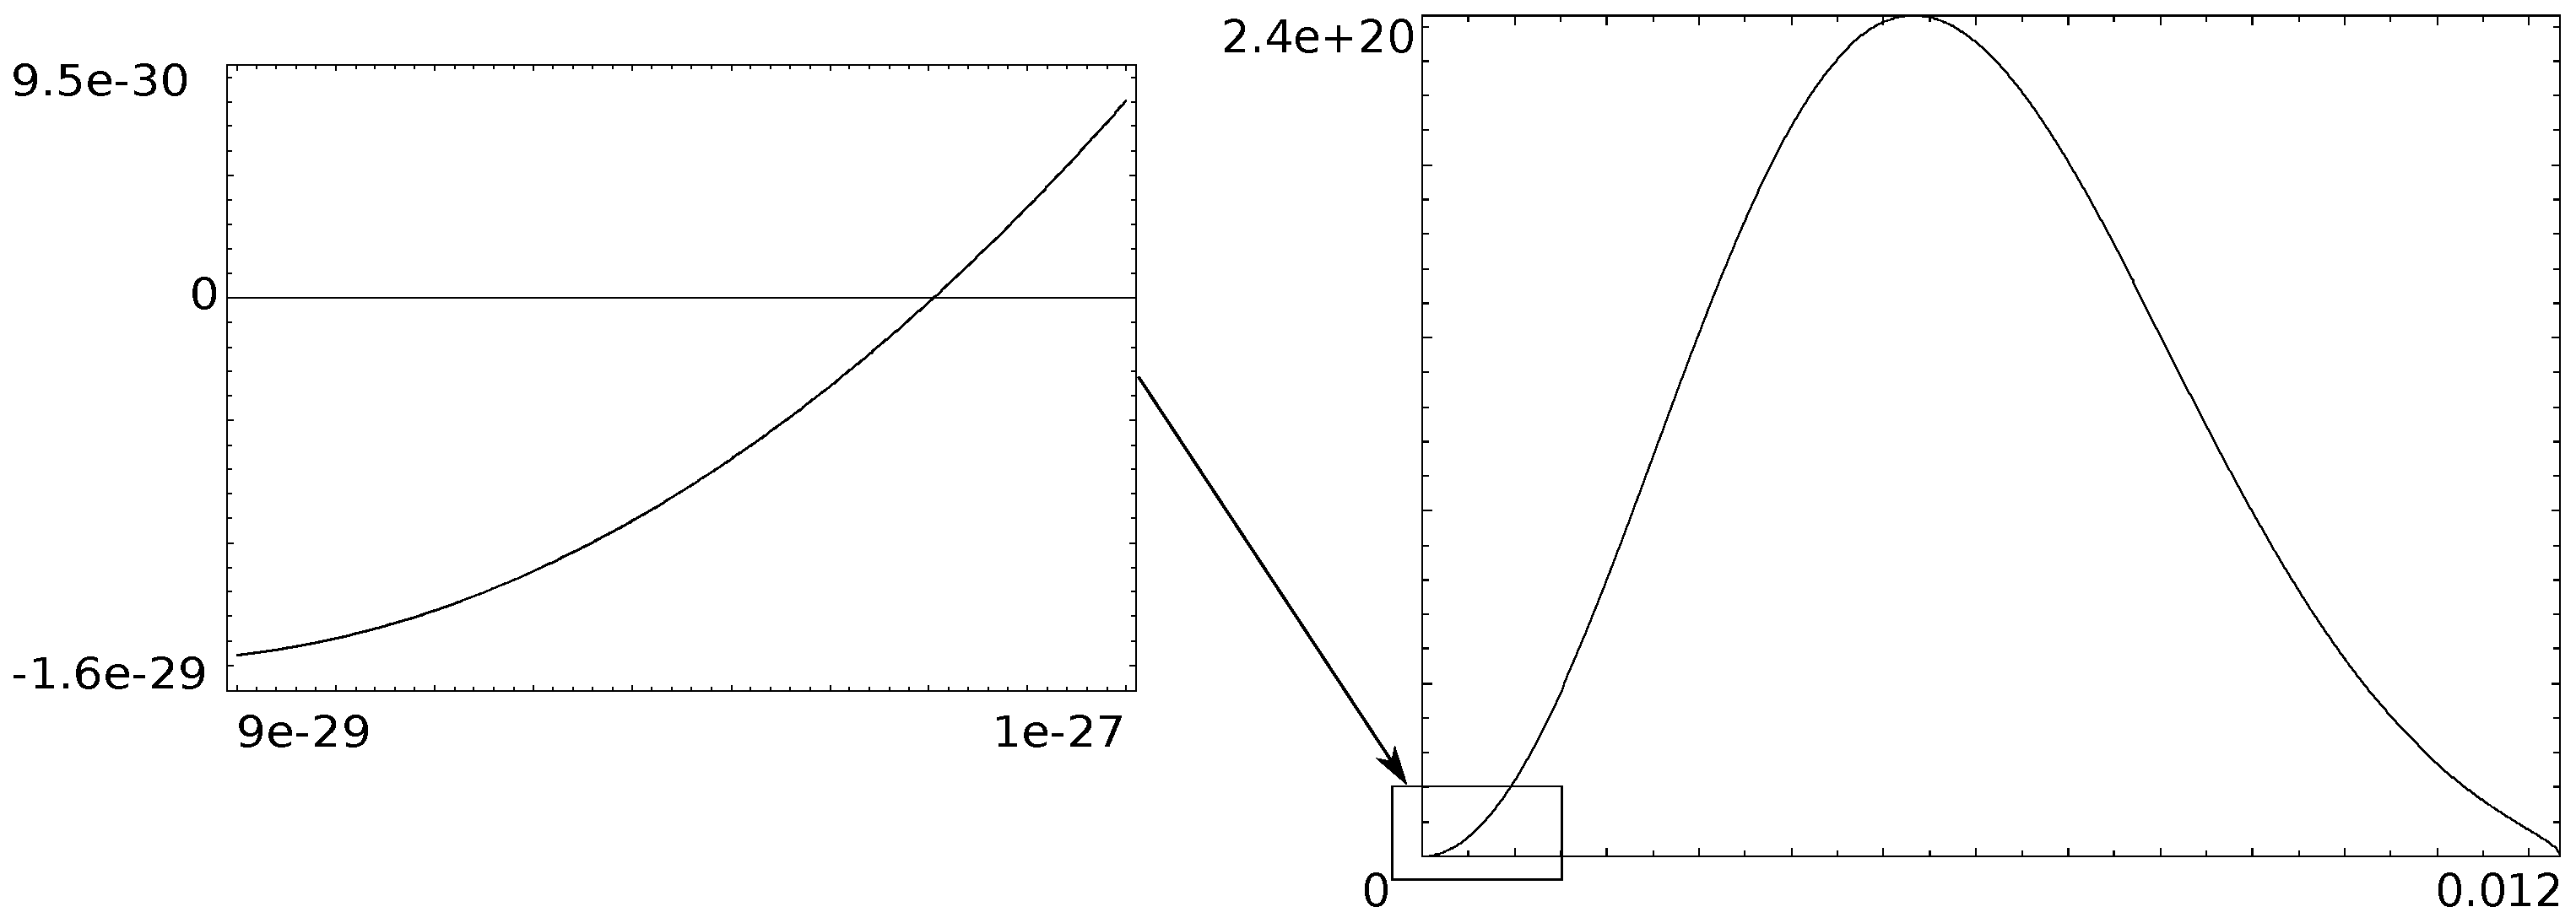
\includegraphics[width=16cm]{full.eps}
 \caption{Левая часть трансцендентного уравнения (\ref{eq:19}) относительно $\lambda$}
 \label{fig2}
\end{figure}
Отметим, что стандартной машинной точности (64--битные числа с плавающей точкой) оказалось недостаточно для нахождения этого корня.
Ввиду этого, для отыскания первого собственного значения использовалась система компьютерной алгебры Pari/GP, 
которая позволяет работать с числами произвольной точности.

\section{Заключение}
Приведенная схема позволяет получать решение задачи методом конечных интегральных преобразований.
При этом основная трудность заключается в поиске корней уравнения (\ref{eq:19}), которые являются
собственными числами задачи Штурма--Лиувилля.

Построенная полная, ортогональная система собственных функций может быть использована в качестве ядер
интегральных преобразований для более сложных: двумерных и трехмерных задач тепло-массопереноса в различных телах.

\section*{Список литерaтуры}
\begin{enumerate}
  \item Беляев Н.М., Рядно А.А. Методы теории теплопроводности.--М.: Высшая школа, 1982.--327с.
  \item Карташов Э.М. Аналитические методы в теории теплопроводности.--М.: Высшая школа, 1985.--480с.
  \item Фарлоу С. Уравнения с частными производными для научных работников и инженеров. --М.: Мир, 1985.--384с.
\end{enumerate}


\end{document}
